\section{Materials}

All solvents were purchased from Sigma-Aldrich and used without any additional treatment.

\Acr{fai}, \acr{mabr} MABr and \acr{mai} were either synthesized in-house (see page \pageref{methods-MAI}) or bought from GreatCell Solar.

 PbI 2 (99 %), PbBr 2 (99.999 %) and CsI (99.999 %) were bought form Sigma-
Aldrich. All of these components are stored in a nitrogen-filled glovebox. The solution for the
dense TiO 2 layer was prepared using 0.65 mL of Ti(IV) isopropoxide (Sigma-Aldrich 97 %) and
0.38 mL of acetylacetone (Sigma-Aldrich) in 5 mL of ethanol. The perovskite (CsFAMAPbIBr)
precursors solution was prepared dissolving 507 mg of PbI 2 , 73.4 mg of PbBr 2 , 172 mg of FAI
and 22.4 mg of MABr in 0.2 mL dimethyl sulfoxide (DMSO) mixed with 0.8 mL of N,N-
dimethylformamide (DMF, anhydrous). The solution was stirred at RT for 1 hour. Then \SI{42}{\micro\litre} of
a 1.5 M CsI solution in DMSO were added to the previous solution. Spiro-OMeTAD (1-Material)
solution was prepared dissolving 72.3 mg in 1 mL of chlorobenzene (anhydrous), then \SI{28.8}{\micro\litre}
of 4-tert-butylpyridine (Sigma-Aldrich) and \SI{17.5}{\micro\litre} of a \SI{520}{\milli\gram\per\milli\litre} of a Lithium bis
trifluoromethylsulfonyl imide (LiTFSI, Sigma-Aldrich) solution in acetonitrile were added. TAE-1
was synthesized as reported 10 and the solution was prepared using the same additives as for
the spiro-OMeTAD solution, but all the molar concentrations halved due to solubility issues.
4
TAE-3 and TAE-4 solutions were prepared with the same additives as for spiro-OMeTAD
solution, but all the molar concentrations reduced to one third for TAE-3 and to one sixth for
TAE-4 due to their lower solubility.

\subsection{Materials handling and purification}


	\subsection{MAI synthesis}\label{methods-MAI}
	
		Reference in laboratory notebook: [ig15, ig18, ig31, ig83].
		
		The synthesis was inspired by \cite{Im2011a, Aharon2014, Williams2014, Etgar2012a, Nagaoka2015}.
		
		In a \SI{500}{\milli\litre} one-necked flask (a big vessel helps later for drying) opened at air, \SI{14}{\milli\litre} of a 40~w/w\% methylamine solution in MeOH (from TCI, ca. 9.8~M) were introduced. Dropwise, \SI{15}{\milli\litre} of hydroiodic acid in water (Aldrich, to be kept in fridge, gets orange with degradation, 57~m/m\%) was added while stirring and cooling at \SI{0}{\celsius}. This mixture was left stirring at room temperature and then still overnight covering the flask neck without completely closing it.
		The solution was evaporated in a vacuum -assisted rotatory evaporator at \SI{60}{\celsius}.
		The obtained white solid was scraped and transferred on a funnel with membrane filter (Sartorius, PTFE). It was washed with diethyl ether and the diethyl ether discarded. The solid was dissolved with ethanol, using as little volume as possible and vacuum was used for forcing the ethanol through the filter. The solid was recrystallized pouring abundant diethyl ether, then filtered, washed with diethyl ether and dried at vacuum.

\section{Perovskite Solar Cells}

	The "top" or "bottom" naming refers to the cell orientation during fabrication, so the "bottom" layer is the one in contact with the glass substrate. 

	\subsection{Top Cathode Perovskite Solar Cells}

		\subsubsection{Anode and HTM substrate preparation}
		
		\subsubsection{MAPI Perovskite Two Step Fabrication}
	
	\subsection{Bottom Cathode Perovskite Solar Cells}
	
		\subsubsection{Cathode and ETM substrate preparation}
	
		\subsubsection{MAPICl Perovskite Two Step Fabrication}
		
		\subsubsection{CsFAMAPbIBr Perovskite One Step Fabrication}
		
		\subsubsection{HTM and cathode deposition}

	\subsection{Handling and Preservation}
		In case of bottom cathode cells, the oxidation of the HTM has been proven to improve the PCE. The oxidation can be induced via a dopant, for example FK209 CITATION, or via oxygen exposure. The latter has to be performed in dark as a synergic light and oxygen contribution on the perovskite layer degradation has been reported CITATION. The oxygen can enter in direct contact with the perovskite layer due to permeability of the HTM; additionally, when a mesoporous ETM is used (e.g. titania) oxygen can diffuse rapidly through the partially infiltrated mesoporous structure. For this reason a cabinet has been modified adding of a constant dry air inlet and physically reducing the leaks of the opening door edges.
				
		\begin{figure}%[!hbtp]%
			\centering
			\begin{subfigure}[b]{0.45\textwidth}
				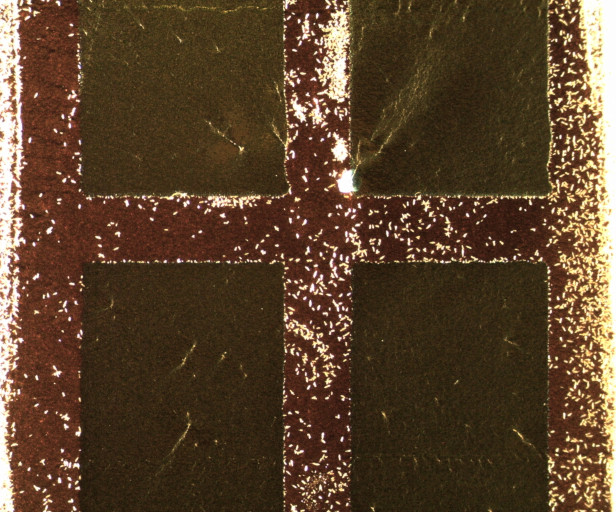
\includegraphics[width=1\textwidth]{microscope_degradation/ig93-1387-1-rescaled.jpg}
				\subcaption{Original cell, gold side.}\label{fig:microscope_degradation-start}
			\end{subfigure}
			\qquad
			\begin{subfigure}[b]{0.45\textwidth}
				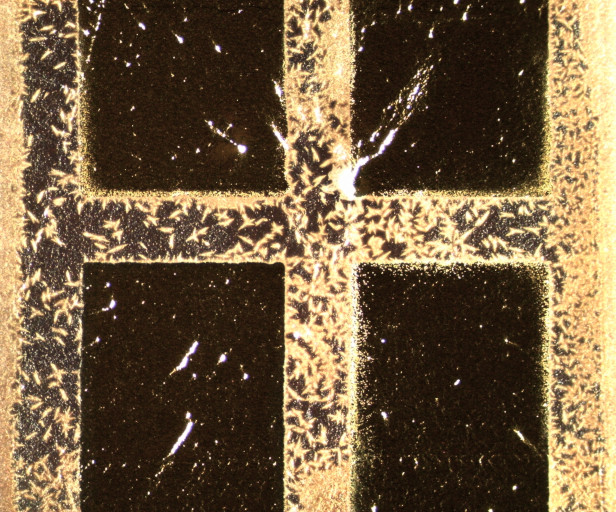
\includegraphics[width=1\textwidth]{microscope_degradation/ig93-1387-8-rescaled.jpg}
				\subcaption{After 10 minutes, gold side.}\label{fig:microscope_degradation-end_front}
			\end{subfigure}
			\bigskip
			
			\begin{subfigure}[b]{0.45\textwidth}
				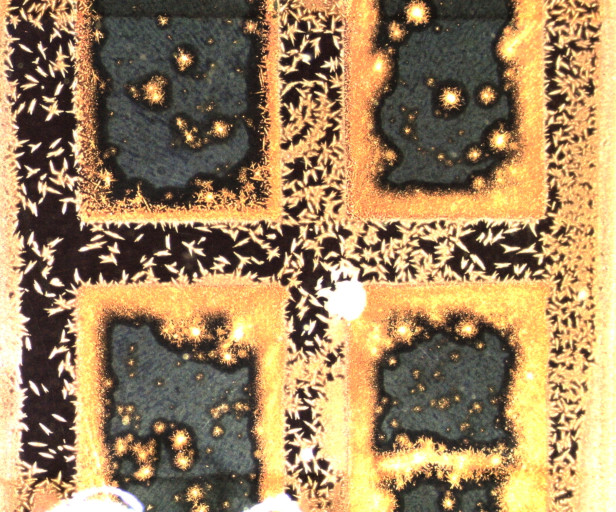
\includegraphics[width=1\textwidth]{microscope_degradation/ig93-1387-back-rescaled.jpg}
				\subcaption{After 10 minutes, glass side.}\label{fig:microscope_degradation-end_back}
			\end{subfigure}
			\caption{Degradation of a FTO/d-TiO$_2$/mp-TiO$_2$/CsFAMAPbIBr/spiro-OMeTAD/Au device upon 10 minutes illumination in air. [ig93]}\label{fig:microscope_degradation}
		\end{figure}
	
		In Fig.~\ref{fig:microscope_degradation} the degradation of a complete device exposed to continuous illumination for 10 minutes and ambient air conditions is shown. An analogous device kept in air but without illumination did not show any degradation as observable via optical microscopy. The gold contact was not enough for protecting the perovskite layer from degradation, as oxygen could penetrate through the mesoporous titania. Interestingly the degradation is more prominent at metallic contacts' edges, one could speculate the reason being the electrical field being higher at smaller curvature metallic edges (seems that there's no therm in English for this, in Italian is referred as "effetto punta" and corona effect concentration ad edges derives from this). It could also be that the ionic profile of perovskite when holes quasi Fermi level is pinned at gold workfunction makes perovskite more sensible to degradation, and this is more evident at edges due to oxygen diffusion being blocked by the gold layer.

		Even if storage in dark and dry air should not be damaging for perovskite solar cells, the most usual long-term storage happens in a nitrogen-filled glovebox.

\section{Solar Cells Characterization}

	All the characterization on complete devices was performed keeping them in a air tight holder filled with nitrogen. The electrical connection from the cell electrode to the external end of the holder was obtained via gold tips connected via a printed circuit board to a coaxial cable.

	\subsection{Current-Voltage Curve}

		


	\subsection{Transient PhotoVoltage}
	
	\subsection{Charge Extraction}
	
	\subsection{Transient PhotoCurrent}
	
	\subsection{Differential Capacitance}
	
\section{Data Analysis and Handling}



